\documentclass[a4paper,12pt]{article}
\usepackage[margin=0.25in]{geometry}
\usepackage{amsmath,amssymb,graphicx,ulem,fancyhdr,fix-cm,xcolor,soul}
\usepackage[utf8]{inputenc}
\usepackage[english]{babel}
\usepackage{xcolor}
\usepackage{lastpage}
\usepackage[english]{babel}
\usepackage{titlesec}

\titleformat{\section}[runin]
{\normalfont\Large\bfseries}{\thesection}{}{}
\definecolor{background}{rgb}{1,1,0.92}
\pagenumbering{arabic}
\graphicspath{ {./images/} }
\setlength\headheight{110pt} 
\pagestyle{fancy}


%document variables 
\newcommand{\SheetNum}{Sheet 3 }
\newcommand{\SheetName}{Bisection \& Fixed Point}
\newcommand{\CourseCode}{CSE 213}
\newcommand{\CourseName}{Numerical Analysis}



\begin{document}
\section*{}%Coverpage
%cover Page,w/ university logo
 \pagecolor{background}
 \fancyhead[R]{ 
\includegraphics[width=12cm]{logo.png}}
 \fancyhead[L]{\fontsize{15}{20} \selectfont \textbf{\CourseCode - \CourseName\\ Spring '22\\ \ \\}}	
	\begin{center}
	\vspace*{6cm}
	\fontsize{40}{60} \selectfont \SheetNum - \SheetName \\
	\fontsize{30}{40}\selectfont \CourseCode - \CourseName \\
	\fontsize{28}{35}\selectfont 120200033 \qquad \ CSE Section 01\\
	\fontsize{25}{30}\selectfont Ahmad Mongy Saad Aboelnaga\\
	\fontsize{20}{25}\selectfont Ahmad.Aboelnaga@ejust.edu.eg	
	\newpage
	\end{center}
	\addtolength{\topmargin}{-.75in}
	\fancyhead[R]{\Large \textbf{\SheetNum}}
	 \fancyhead[L]{\fontsize{18}{20} \selectfont \CourseCode - \CourseName, Spring '22}
\section*{\LARGE Question 2:}{ \LARGE For root finding – Textbook (9\textsuperscript{th} edition) – Problem Set 2.2 (Page 64). Problems 12 b) and d) are to do as homework.}\\[0.5cm]
\Large \textbf{12.} For each of the following equations, use the given interval or determine an interval [a, b] on which fixed-point iteration will converge. Estimate the number of iterations necessary to obtain approximations accurate to within $10^{-5}$, and perform the calculations.\\ 

\textbf{b.} $x^3 - 2x - 5 = 0 $ \hspace{4.8cm} use [2,3] \vspace{0.4cm}

{\color{blue}Solution:\\ $ \indent \qquad g_1(x) = \dfrac{x^3-5}{2}$ \hspace{0.5cm} or \hspace{0.5cm} $g_2(x) = \sqrt[3]{2x+5}$\\

$\indent \qquad $
\begin{tabular}{|c|c|c|}
\hline 
$g(x) $   & $g_1(x)= \dfrac{x^3-5}{2}$ & $g_2(x)= \sqrt[3]{2x+5}$ \\ 
\hline 
$g'(x)$ & $g'_1(x)= \dfrac{3x^2}{2} $ & $g'_2(x)=\dfrac{2}{3(2x+5)^\frac{2}{3}}$ \\ 
\hline 
max($|k|$) & {\color{red} 13.5 (not acceptable)} & {\color{cyan} 0.15408028319} \\ 
\hline 
\end{tabular} \\[0.5cm]
\begin{align*}
n &> \dfrac{ln(10^{-5})-ln(max(p_0 -a,b-p_0))}{ln(k)}\\
n &> \dfrac{ln(10^{-5})-ln(1)}{ln(0.15408028319)}\\
n &> 6.1557\\
\end{align*}
$\therefore$ we expect $n > 6$, however; the desired tolerance is met with exactly 6 iterations.
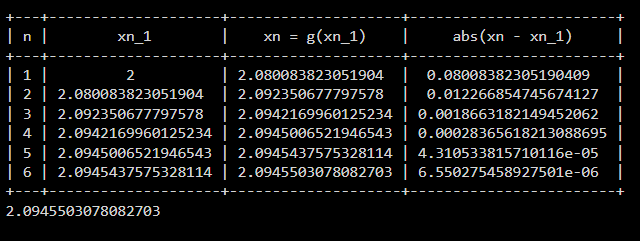
\includegraphics[scale=1.5]{Q2 b.png}
\color{black}
\newpage
\textbf{d.} $x - \cos (x)  = 0 $ \hspace{4.8cm} using [0,1] \vspace{0.4cm}

{\color{blue}Solution:\\ $ \indent \qquad g_1(x) = \cos(x)$ \hspace{0.5cm} or \hspace{0.5cm} $g_2(x) = \cos^{-1}(x)$\\

$\indent \qquad $
\begin{tabular}{|c|c|c|}
\hline 
$g(x) $   & $g_1(x)= \cos(x)$ & $g_2(x)= \cos^{-1}(x)$ \\ 
\hline 
$g'(x)$ & $g'_1(x)= -\sin(x) $ & $g'_2(x)=\dfrac{1}{\sqrt{1-x^2}}$ \\ 
\hline 
max($|k|$) & {\color{cyan} 0.84147098481 } & {\color{red} $\infty$ (not acceptable)} \\ 
\hline 
\end{tabular} \\[0.5cm]
\begin{align*}
n &> \dfrac{ln(10^{-5})-ln(max(p_0 -a,b-p_0))}{ln(k)}\\
n &> \dfrac{ln(10^{-5})-ln(1)}{ln(0.84147098481)}\\
n &> 66.70148078\\
\end{align*}
$\therefore$ we expect $n > 66$, however; the tolerance is met with exactly 30 iterations.
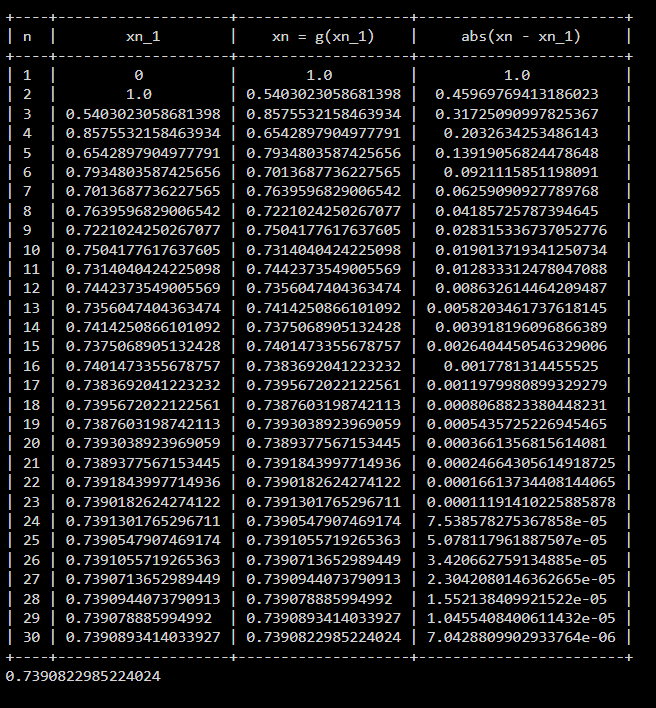
\includegraphics[scale=1]{Q2 d.png}
\color{black}
\newpage
Tools used in creating this document:
 \begin{itemize}
 \item Texmaker 5.0.4
 \item Google Colab with python 3.7.13 [GCC 7.5.0]
\end{itemize}  
 
 \copyright All questions in this file has been adapted from the sheet provided by the course instructor, I have only reorganized the sheet and attempted to answer it. Please do not share without the permission of the owner.\\
\color{blue}Ahmad.Aboelnaga@ejust.edu.eg\\
ID:120200033, CSE01
 
  
\end{document}			
